%-------------------------------------------------------------------------------
%                            BAB II
%               TINJAUAN PUSTAKA DAN DASAR TEORI
%-------------------------------------------------------------------------------
\fancyhf{} 
\fancyfoot[C]{\thepage}
\chapter{TINJAUAN KEPUSTAKAAN}               

\section{\uppercase{Hidroponik}}
Istilah hidroponik (Inggris: \textit{hydroponic}) berasal dari kata Yunani yaitu \textit{hydro} yang berarti air dan \textit{ponos} yang berarti daya. Hidroponik juga dikenal sebagai \textit{soilless culture} atau budi daya tanaman tanpa tanah. Secara umum, hidroponik merupakan budi daya menanam tanpa tanah, akan tetapi dengan memanfaatkan air dan lebih menekankan pada pemenuhan kebutuhan nutrisi tanaman \citep{alviani2015bertanam}.

\par Hidroponik mempunyai berbagai kelebihan apabila dibandingkan dengan bercocok tanam sistem konvensial, antara lain adalah tidak menuntut lahan yang luas sehingga mungkin diterapkan oleh masyarakat perkotaan dengan ketersediaan lahan kosong yang terbatas, lokasi penanaman bisa di mana saja, pilihan jenis tanaman yang bisa ditanam sangat beragam, tingkat pertumbuhan yang lebih cepat sehingga lebih cepat dipanen, dan teknis perawatannya relatif tidak sulit sehingga bisa dipraktikkan oleh hampir semua orang \citep{iqbal2016simpel}.

\section{\uppercase{Pemasaran Digital}}
Pemasaran digital adalah suatu usaha untuk mempromosikan sebuah merek dengan menggunakan media digital yang dapat menjangkau konsumen secara tepat waktu, pribadi, dan relevan. Tipe pemasaran digital mencakup banyak teknik dan praktik yang terkandung dalam kategori pemasaran internet. Dengan adanya ketergantungan pemasaran tanpa internet membuat bidang pemasaran digital menggabungkan elemen utama lainnya seperti ponsel, SMS (pesan teks dikirim melalui ponsel), menampilkan iklan spanduk, dan digital luar. \citep{wikipedia2021}

\par Pemasaran digital adalah salah satu media pemasaran yang saat ini sedang banyak diminati oleh masyarakat untuk mendukung berbagai kegiatan yang dilakukan. Mereka sedikit demi sedikit mulai meninggalkan model pemasaran konvesional/tradisional beralih ke pemasaran moderen yaitu pemasaran digital. Dengan pemasaran digital komunikasi dan transaksi dapat dilakukan setiap waktu/\textit{real time} dan bisa mengglobal atau mendunia. Dengan jumlah pengguna media sosial berbasis \textit{chat} ini yang banyak dan semakin hari semakin bertambah membuka peluang bagi UKM untuk mengembangkan pasarnya dalam genggaman \textit{smartphone} \citep{pradiani2017pengaruh}.

\section{\uppercase{E-commerce}}
\textit{E-commerce} (\textit{Elektronic Commerce}) atau dalam bahasa indonesia perdagangan secara elektronik adalah aktivitas penyebaran, penjualan, pembelian, pemasaran produk (barang dan jasa), dengan memanfaatkan jaringan telekomunikasi seperti internet, televisi, atau jaringan komputer lainnya. Secara sederhana \textit{e-commerce} adalah proses pembelian maupun penjualan produk secara elektronik. \textit{E-commerce} sendiri semakin kian berkembang beberapa tahun belakangan ini dan secara perlahan menggantikan toko tradisional (\textit{offline}) \citep{idcloudhost2021}.

\section{\uppercase{Website}}
\textit{World Wide Web} atau yang lebih dikenal dengan istilah web (\textit{website}) adalah sistem pengakses informasi dalam internet \citep{abdul2014pengenalan}. Web disusun dari halaman – halaman yang menggunakan teknologi web dan saling berkaitan satu sama lain. Sedangkan pengertian lain menyebutkan bahwa website adalah rangkaian atau sejumlah halaman web di internet yang memiliki topik saling berkaitan untuk mempresentasikan suatu informasi \citep{ginanjar2014rahasia}.

\par \textit{Website online} harus memiliki domain. Sebuah domain atau alamat web dibuat dengan menggunakan “\textit{Domain Name System}” yang merupakan metode yang dipakai untuk mengorganisir seluruh nama – nama komputer yang ada di internet. Contoh domain adalah .com (komersil atau bisnis), .gov (pemerintahan), .mil (militer), .net (intitusi yang berbeda), dan .ac (institusi pendidikan). Untuk top domain .id (Negara Indonesia), .ca (Negara Canada), .us (Negara Amerika) dan sebagainya yang berarti kepemilikan web negara \citep{dhika2015perancangan}.

\section{\uppercase{Entity Relationship Diagram (ERD)}}
Menurut \cite{priyadi2014} menyatakan bahwa : Pemodelan basis data dengan menggunakan diagram relasi antara entitas, dapat dilakukan dengan menggunakan suatu pemodelan basis data yang bernama Diagram \textit{Entity Relationship} yang disingkat Diagram E-R. ERD juga merupakan gambaran yang menghubungkan antara objek satu dengan objek yang lain dalam dunia nyata. Bisa dikatakan bahwa bahan yang akan digunakan untuk membuat ERD adalah dari objek di dunia nyata. Secara umum ERD terdiri dari 4 komponen, yakni :

\begin{enumerate}
	\item Entitas
	\par Entitas merupakan notasi untuk mewakili suatu objek dengan karakteristik sama, yang dilengkapi oleh atribut, sehingga pada suatu lingkungan nyata objek akan berbeda dengan objek lainnya.
	\item Relasi
	\par Relasi merupakan notasi yang digunakan untuk menghubungkan beberapa entitas berdasarkan fakta pada suatu lingkungan.
	\item Atribut
	\par Atribut merupakan notasi yang menjelaskan karakteristik suatu entitas dan juga relasinya. Atribut dapat sebagai \textit{key} yang bersifat unik, yaitu \textit{primary key} atau \textit{foreign key}. Selain itu, atribut juga dapat sebagai atribut deskriptif saja, yaitu sebagai pelengkap deskripsi suatu entitas dan relasi.	
	\item Garis Penghubung
	\par Garis penghubung merupakan notasi untuk merangkai keterkaitan antara notasi-notasi yang digunakan dalam Diagram E-R , yaitu entitas, Relasi , dan atribut.
\end{enumerate}

\section{\uppercase{Laravel Livewire}}
Laravel merupakan sebuah kerangka kerja yang dikembangkan oleh Taylor Otweel di MIT dengan basis bahasa pemograman PHP (\textit{Hypertext Preprocessor}) yang bersifat \textit{Open Source} dimana Laravel ini menggunakan kerangka arsitektur MVC (\textit{Model-View-Controller}) dimana komponen pada Laravel sangat mudah untuk dipahami seperti fitur \textit{authentication}, \textit{session manager}, \textit{routing}, dan \textit{caching}, kemudian fitur Unit Testing \textit{Support} yang telah terintegrasi untuk seorang pengembang laman web agar lebih mudah dalam mengembang aplikasi yang kompleks \citep{sebastian2021perancanagan}.

\par Livewire adalah kerangka kerja \textit{full-stack} untuk kerangka Laravel yang membuat membangun antarmuka dinamis menjadi sederhana, tanpa meninggalkan kenyamanan Laravel. Jika Anda menggunakan Livewire dengan Laravel maka Anda tidak perlu khawatir tentang menulis kode Ajax jQuery, Livewire akan membantu menulis kode Ajax jQuery dengan cara yang sangat sederhana menggunakan PHP tanpa penyegaran halaman Validasi Laravel akan berfungsi, formulir akan dikirimkan, dll. Apa yang dilakukan Laravel Livewire? \citep{krishaweb2021}

\begin{itemize}
	\item Livewire merender \textit{output} komponen awal dengan halaman (seperti \textit{Blade} termasuk), dengan cara ini SEO \textit{friendly}.
	\item Ketika interaksi terjadi, Livewire membuat permintaan AJAX ke server dengan data yang diperbarui.
	\item Server merender ulang komponen dan merespons dengan HTML baru.
	\item Livewire kemudian dengan cerdas mengubah DOM sesuai dengan hal-hal yang berubah.
\end{itemize}

\begin{figure}[H]
\centering
{
\includegraphics [width = 10.5cm, height= 6cm]{gambar/laravel-livewire}}
\caption{Laravel Livewire \citep{krishaweb2021}}
\label{laravel_livewire}
\end{figure}

\section{\uppercase{MySQL}}
MySQL adalah salah satu program yang dapat digunakan sebagai \textit{database}, dan merupakan salah satu \textit{software} untuk \textit{database} server yang banyak digunakan. MySQL bersifat \textit{open source} dan menggunakan SQL. MySQL bisa dijalankan diberbagai platform misalnya Windows, Linux, dan lain sebagainya. MySQL memiliki kelebihan, antara lain: \citep{orlando2017aplikasi}

\begin{enumerate}
	\item Dapat digunakan oleh beberapa \textit{user} dalam waktu yang bersamaan tanpa mengalami masalah.	
	\item Memiliki kecepatan yang bagus dalam menangani \textit{query} sederhana.
	\item Memiliki operator dan fungsi secara penuh dan mendukung perintah \textit{select} dan \textit{where} dalam perintah \textit{query}.
	\item Memiliki keamanan yang bagus karena beberapa lapisan sekuritas seperti level \textit{subnetmask}, nama \textit{host}, dan izin akses \textit{user} dengan sistem perizinan yang mendetail serta sandi terenkripsi.
	\item Mampu menangani basis data dalam skala besar, dengan jumlah rekaman lebih dari 50 juta dan 60 ribu tabel serta kurang lebih 5 milyar baris. Selain itu batas indeks yang dapat ditampung mencapai 32 indeks pada tiap tabelnya
\end{enumerate}

\section{\uppercase{Web Service}}
\textit{Web service} adalah salah satu bentuk sistem perangkat lunak yang didesain untuk mendukung interaksi mesin ke mesin melalui jaringan. \textit{Web service} memiliki \textit{interface} yang dideskripsikan dalam format yang dapat dibaca oleh mesin \citep{prabowo2016teknologi}. Kasman mengemukakan, “\textit{Web Service} adalah aplikasi yang dibuat agar dapat dipanggil dan diakses oleh aplikasi lain melalui internet dengan menggunakan format pertukaran data sebagai format pengiriman pesan” \citep{kasman2015}. \textit{Web service} digunakan sebagai salah satu fasilitas yang disediakan oleh suatu web untuk menyediakan layanan dalam bentuk informasi kepada sistem lain, sehingga sistem lain dapat berinteraksi dengan sistem tersebut melalui layanan \textit{service} yang disediakan oleh suatu sistem yang menyediakan \textit{web service}.” Pada penelitian ini akan digunakan \textit{web services} dengan layanan protokol REST untuk membantu aplikasi penjualan tanaman hidroponik berbasis Android berinteraksi dengan \textit{database} yang terdapat di web server.

\section{\uppercase{REST}}
REST (\textit{Representational State Transfer}) merupakan standar arsitektur komunikasi berbasis web yang sering diterapkan dalam pengembangan layanan berbasis web atau sistem terdistribusi. RESTful \textit{web service} atau juga dikenal dengan nama RESTful Web API merupakan sebuah \textit{web service} yang di implementasikan dengan menggunakan HTTP dengan menggunakan prinsip-prinsip REST. Istilah REST diperkenalkan oleh Roy Fielding pada tahun 2000. Arsitektur gaya REST adalah arsitektur klien server di mana klien mengirim permintaan ke server, server kemudian memproses permintaan dan mengembalikan tanggapan. Umumnya menggunakan HTTP (\textit{Hypertext Transfer Protocol}) sebagai protokol untuk komunikasi data \citep{saputra2018}.

\par Berikut metode HTTP yang umum digunakan dalam arsitektur berbasis REST:
\begin{enumerate}
	\item GET, menyediakan hanya akses baca pada \textit{resource}.
	\item PUT, digunakan untuk menciptakan \textit{resource} baru.
	\item DELETE, digunakan untuk menghapus \textit{resource}.
	\item POST, digunakan untuk memperbarui \textit{resource} yang ada atau membuat \textit{resource} baru.
	\item OPTIONS, digunakan untuk mendapatkan operasi yang di \textit{support} pada \textit{resource}.
\end{enumerate}

\section{\uppercase{Virtual Private Server (VPS)}}
\textit{Virtual Private Server} (VPS) adalah \textit{virtual machine} yang dijual sebagai layanan oleh \textit{hosting provider}, dalam VPS \textit{user} bisa mengakses dan mengelola seluruh aspek \textit{software} dari server termasuk akses administrator di sistem oprasi server sampai aplikasi yang akan di implementasikan di server tersebut. VPS dapat dibagi menjadi beberapa VM \textit{(Virtual Machines)}, dimana di setiap VM adalah berupa \textit{“Virtual server”} yang dapat di \textit{install} sistem operasi tersendiri. VPS terasa seperti sebuah \textit{Dedicated Server}. Dibanding dengan \textit{shared hosting}, menyewa VPS akan mendapatkan \textit{resource} yang lebih baik sehingga tidak terganggu jika ada problem pada \textit{website} yang dikelola. Selain itu VPS mendapatkan \textit{root} akses sehingga lebih leluasa dalam mengkustomasi server sesuai kebutuhan \citep{hamida2017analisis}.

\section{\uppercase{Scrum}}
\textit{Scrum} dikembangkan oleh Jeff Sutherland pada tahun 1993 untuk menciptakan metode pengembangan yang mengikuti prinsip-prinsip metode \textit{Aglie} \citep{fernando2018rancang}. \textit{Scrum} merupakan satu metode \textit{agile} paling popular. Metode ini merupakan metode adaptif, cepat, fleksibel, dan efektif serta dapat memberikan hasil yang signifikan dengan cepat \citep{hadinata2017implementasi}. \textit{Scrum} adalah sebuah kerangka kerja untuk pengembangan tambahan yang menggunakan satu atau lebih tim \textit{cross} fungsional. \textit{Scrum} menggunakan iterasi tetap yang disebut \textit{sprint}, yang berlangsung selama satu hingga empat minggu. Tim \textit{scrum} berusaha untuk menghasilkan peningkatan yang telah diuji disetiap iterasi. Alur metode \textit{scrum} dapat dilihat pada gambar 2.2.

\begin{figure}[H]
\centering
{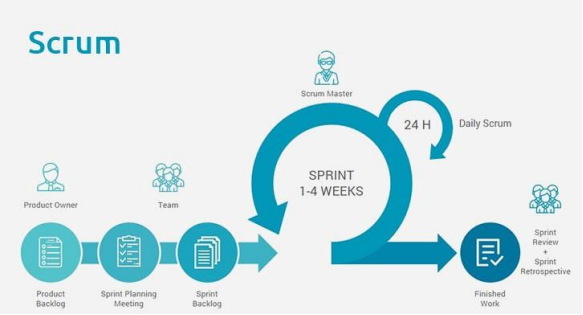
\includegraphics [width = 12.5cm, height= 7cm]{gambar/scrum}}
\caption{Metode Scrum \citep{wahyudi2018analisis}}
\label{scrum}
\end{figure}	

\par \textit{Scrum} menurut \citep{wahyudi2018analisis} adalah salah satu metode pengembangan aplikasi dengan pengimplementasian proses \textit{Agile Development}. \textit{Scrum} mempunyai perbedaan yang signifikan dikarenakan produk yang dihasilkan akan menyesuaikan dengan lingkungan seiring waktu proses pengembangan berlalu.

\section{\uppercase{Black Box Testing}}
\textit{Black Box Testing} berfokus pada pengujian dari masing-masing spesifikasi fungsional perangkat lunak. Seorang tester dapat mendefinisikan kumpulan kondisi \textit{input} dan melakukan pengetesan pada fungsionalitas perangkat lunak \citep{mustaqbal2015pengujian}. Metode \textit{Black Box testing} terdiri atas beberapa metode, antara lain \textit{Equivalence Partitioning}, \textit{Boundary Value Analysis}, \textit{State Transition Testing}, dan \textit{Decision Table Testing}.

\par \textit{Black Box Testing} merupakan metode pengujian perangkat lunak yang digunakan untuk menguji sebuah perangkat lunak tanpa 
mengetahui struktur internal kode atau program. Dalam pengujiannya, penguji menyadari apa yang harus dilakukan oleh program, tapi tidak memiliki pengetahuan tentang bagaimana melakukannya. Kelebihan \textit{black box testing} yaitu :

\begin{enumerate}
	\item Efisien untuk segmen kode besar.
	\item Akses kode tidak diperlukan.
	\item Pemisahan antara perspektif pengguna dan pengembang.
\end{enumerate}

\par Selain memiliki kelebihan, \textit{black box testing} juga memiliki kelemahan, yaitu:

\begin{enumerate}
	\item Cakupan terbatas karena hanya sebagian kecil dari skenario pengujian yang dilakukan. 
	\item Pengujian tidak efisien karena keberuntungan tester dari pengetahuan tentang perangkat lunak internal.
\end{enumerate}

\section{\uppercase{System Usability Scale (SUS)}}
\textit{System Usability Scale} (SUS) adalah salah satu metode uji pengguna yang menyediakan alat ukur yang “\textit{quick and dirty}” yang dapat diandalkan. Metode uji pengguna ini diperkenalkan oleh John Brooke pada tahun 1986 \citep{thomas2015use} yang dapat digunakan untuk melakukan evaluasi berbagai jenis produk ataupun layanan, termasuk di dalamnya \textit{hardware}, \textit{software}, perangkat \textit{mobile}, \textit{website}, dan aplikasi.

\textit{System Usability Scale} (SUS) merupakan metode evaluasi kegunaan yang memberikan hasil yang memadai berdasarkan pertimbangan 
jumlah sampel yang kecil, waktu, dan biaya. Hasil dari perhitungan dengan menggunakan metode SUS akan dikonversi ke dalam sebuah 
nilai, yang dapat dijadikan pertimbangan utuk menentukan apakah sebuah aplikasi layak atau tidak layak untuk diterapkan. \citep{pudjoatmodjo2016tes}

\par Metode penilaian \textit{System Usability Scale} mengharuskan para peserta untuk memberikan tanggapan terhadap 10 item pernyataan menggunakan 5 poin skala \textit{Likert}. Responden diminta untuk memberikan penilaian dari skala 1 yang berarti “Sangat tidak setuju”, skala 2 yang berarti “Tidak setuju”, skala 3 yang berarti “Netral”, skala 4 yang berarti “Setuju”, dan skala 5 yang berarti “Sangat setuju”. Jika karena alasan tertentu, Jika responden merasa tidak menemukan skala respon yang tepat, responden harus mengisi titik tengah skala pengujian. \textit{System Usability Scale} dipercaya skala yang dapat digunakan untuk dua faktor yang berbeda, yaitu mengukur keseluruhan dari \textit{usability} (8 dari 10 item) dan mengukur \textit{learnability} 
(2 dari 10 item) dari suatu sistem. Adapun daftar pertanyaan SUS dapat dilihat pada Tabel 2.1.

\begin{table}[H]
\centering
\caption{Daftar Pertanyaan Metode SUS \citep{kortum2015measuring}}
\label{item_pernyataan_system_usability_scale}
\begin{tabular}{|l| >{\centering\arraybackslash} m{12cm}|} 
\hline
\textbf{No.} & \textbf{Pertanyaan}  \\ 
\hline
1.           &  Saya akan ingin lebih sering menggunakan aplikasi ini   \\ 
\hline
2.           & Saya merasa aplikasi ini tidak harus dibuat serumit ini  \\ 
\hline
3.           & Saya pikir aplikasi ini mudah untuk digunakan  \\ 
\hline
4.           & Saya membutuhkan bantuan dari orang teknis untuk menggunakan aplikasi ini    \\ 
\hline
5.           & Saya menemukan fitur pada aplikasi terintegrasi dengan baik   \\
\hline
6.           & Saya merasa banyak hal-hal yang tidak sesuai (tidak konsisten) pada aplikasi ini   \\
\hline
7.           & Saya merasa orang lain dapat belajar cara menggunakan aplikasi ini dengan cepat   \\
\hline
8.           & Saya merasa aplikasi ini membingungkan   \\
\hline
9.           & Saya merasa percaya diri (nyaman) dalam menggunakan aplikasi ini   \\
\hline
10.           & Saya perlu belajar banyak hal terlebih dahulu sebelum menggunakan aplikasi ini   \\
\hline
\end{tabular}
\end{table}

%-----------------------------------------------------------------------------%

% Baris ini digunakan untuk membantu dalam melakukan sitasi
% Karena diapit dengan comment, maka baris ini akan diabaikan
% oleh compiler LaTeX.

\fancyhf{} 
\fancyfoot[R]{\thepage}

\begin{comment}
\bibliography{daftar-pustaka}
\end{comment}
